\documentclass{article}

% Language setting
% Replace `english' with e.g. `spanish' to change the document language
\usepackage[portuguese]{babel}

% Set page size and margins
% Replace `letterpaper' with `a4paper' for UK/EU standard size
\usepackage[letterpaper,top=2cm,bottom=2cm,left=3cm,right=3cm,marginparwidth=1.75cm]{geometry}

% Useful packages
\usepackage{amsmath}
\usepackage{graphicx}


\title{MAP2212 - Exercício de Programação 2}
\author{Lucas Panfilo Donaire - 12556552}

\begin{document}
\maketitle

\newcommand{\PR}[1]{\ensuremath{\left[#1\right]}}
\newcommand{\PC}[1]{\ensuremath{\left(#1\right)}}
\newcommand{\chav}[1]{\ensuremath{\left\{#1\right\}}}

\begin{abstract}
Usando métodos de Monte Carlo para estimar computacionalmente uma integral.
\end{abstract}

\section{Introdução}
\subsection{Métodos de Monte Carlo}

A Lei dos grandes números, ideia fundamental da teoria da probabilidade, foi primeiramente formulada por Jacob Bernoulli: "Para um grande número de experiências, tendo cada uma um resultado aleatório, a frequência relativa de cada um desses resultados tende a estabilizar, convergindo para um certo número que constitui a probabilidade desse resultado".

Disso concluimos que, quando repetimos um experimento, na medida que o número de tentativas aumenta, a média aritmética dos resultados do experimento tende a se aproximar de seu valor esperado. 

Assim surgem os chamados Métodos de Monte Carlo, métodos que usam amostragens aleatórias massivas para obter resultados numéricos sobre alguma distribuição. Tais métodos são úteis para obter aproximações numéricas.

\subsection{f(x)}
Temos que $f = e^{-0.57892819x}\times cos(0.47410024895x)$, e queremos 
\[ 
\gamma = \int_{0}^{1} f(x) \,dx 
\]

Vamos usar 4 métodos distintos para esssa simulação.
\subsection{Alguns resultados que iremos usar}

\subsubsection{Teorema central do limite}

Sejam $X_1, X_2, \ldots, X_n$ uma amostra aleatória simples da população $X$, tal que $\text{E}[X_i] = \mu$ e $\text{Var}[X_i] = \sigma^2 < \infty$. Seja
\[
X_m = \frac{X_1 + X_2 + \cdots + X_n}{n}
      = \frac{1}{n}\sum_{i}^{n} X_i
\]
a média amostral da amostra. Então, conforme $n$ tende a infinito, a variável aleatória $X_m$ converge para uma distribuição normal $\mathcal{N}(\mu, \sigma^2/n)$.

\subsubsection{Tamanho de amostras de distribuições normais}

Suponha que estejamos estimando a média $\mu$ populacional para tanto usaremos a média amostral, $X_m$, baseada numa amostra de tamanho n. Suponha
que se queira determinar o valor de n de modo que 
\[
P(|X_m - \mu| \leq \varepsilon) \geq \delta 
\] 

Com $0 < \delta < 1$, e $\varepsilon$ é o erro amostral máximo que podemos suportar, ambos valores fixados.

Sabemos que $X_m$ tem distribuição $\mathcal{N}(\mu, \sigma^2/n)$. Então:
\[
P(-\varepsilon \leq X_m - \mu \leq \varepsilon) = P(\frac{-\varepsilon \sqrt{n}}{\sigma} \leq Z \leq \frac{\varepsilon \sqrt{n}}{\sigma} ) \approx \delta ,  \]

com Z = $\frac{(X_m - \mu)\sqrt{n}}{\sigma} $.
Dado $\delta$ , podemos obter $z_\delta$ da $\mathcal{N}(0,1)$ tal que $P(-z_\delta \leq Z \leq z_\delta)=\delta$. Assim, temos
\begin{equation}
   z_\delta = \frac{\varepsilon \sqrt{n}}{\sigma} \implies
n = \frac{z_\delta^2 \sigma^2}{\varepsilon^2}
\end{equation}

\subsubsection{Método da transformação inversa}
Resultado: Seja $U \sim U(0,1).$ Para qualquer função f de distribuição acumulada F, a v.a. X definida por
$X=F^{-1} (U)$
possui distribuição f, onde $F^{-1}$ é a inversa generalizada de F.
É simples verificar o seguinte resultado acima. Em geral, observe que
\[
P(X \leq x)= P(F^{-1} (U) \leq x)= P(U \leq F(x)) = F(x).
\]
Logo $X \sim f$.
\subsubsection{Somas da Integral de Darboux}

A integral de Darboux é equivalente à de Riemann e construída a partir de duas somas, uma soma inferior que é sempre menor que a integral, e uma soma superior que é sempre maior. Definição: 

Seja $P = \PC{x_0, x_1,..., x_n}$ uma partição de \PR{a,b}. 
\\
Seja $M_i = sup(f(x)), x \in [x_{i-1}, x_i]$, para i = 1,2,..,n \\
Seja $m_i = inf(f(x)), x \in [x_{i-1}, x_i],$ para i = 1,2,..,n \\
A soma Darboux superior de f em relação a P é: 

\[
U_{f,P} = \sum_{i=1}^{n} (x_i - x_{i-1})M_i 
\]
E a soma Darboux inferior de f em relação a P é:
\[
L_{f,P} = \sum_{i=1}^{n} (x_i - x_{i-1})m_i 
\]
Temos que, para qualquer partição P de (a,b), vale:
\[
U_{f,P} \leq \int_{a}^{b} f(x)dx \leq  L_{f,P}
\]
Isso será útil para calcular limitantes superiores e inferiores da integral que queremos estimar.

\section{Apresentando os métodos}
\subsection{Método de Monte Carlo 'Cru'}
Vamos simular $n_1$ valores $x \sim U(0,1)$, e nosso estimador $\widehat{\gamma_1}$ será calculado como:
\[
\widehat{\gamma_1} = \frac{1}{n_1} \sum_{i=1}^{n_1} f(x_i).
\]
Temos que:
\[ 
E(\widehat{\gamma_1}) = \gamma
\] 
e
\[
\sigma^2_1 = \frac{1}{n_1} \int_{0}^{1} (f(x) - \gamma)^2 \,dx 
\]


\subsection{Método de Monte Carlo 'Hit or Miss'}
Nosso estimador $\widehat{\gamma_2}$

Vamos simular $n_2$ valores $x,y \sim U(0,1)$, e nosso estimador $\widehat{\gamma_2}$ será calculado como:
\[
\widehat{\gamma_2} = \frac{1}{n_2} \sum_{i=1}^{n_2} Ind(y_i \leq f(x_i))
\]
Temos que:
\[ 
E(\widehat{\gamma_2}) = \gamma
\] 
e
\[
\sigma^2_2 = \frac{\gamma(1 - \gamma)}{n_2} 
\]

\subsection{Método de Monte Carlo 'Importance Sampling'}
Tomaremos uma função g(x) que é aproximadamente proporcional a f(x) no intervalo selecionado tal que a integral de g(x) nesse intervalo é igual a 1. Faremos isso para usar g como função de densidade de probabilidade. Temos então:
\[
\int_{0}^{1} f(x) \,dx = \int_{0}^{1} \frac{f(x)}{g(x)}g(x)\,dx 
\]
Assim, vamos simular $n_3$ valores $x \sim g(x)$, e nosso estimador $\widehat{\gamma_3}$ será calculado como:
\[
\widehat{\gamma_3} = \frac{1}{n_3} \sum_{i=1}^{n_3} \frac{f(x_i)}{g(x_i)}.
\]
Temos que:
\[ 
E(\widehat{\gamma_3}) = \gamma
\] 
e
\[
\sigma^2_3 = \frac{1}{n} \int_{0}^{1} (\frac{f(x)}{g(x)} - \gamma)^2 \,g(x)dx
\]
No nosso caso, vamos usar 
\[
g(x) = \frac{4}{3} - \frac{2x}{3}
\]
Achamos essa função 'no olho', e ela é aproximadamente proporcional (imagem 1) a f(x) e tem integral igual a 1 no intervalo [0,1], então ela será nossa função densidade.

\begin{figure}[ht]
\centering
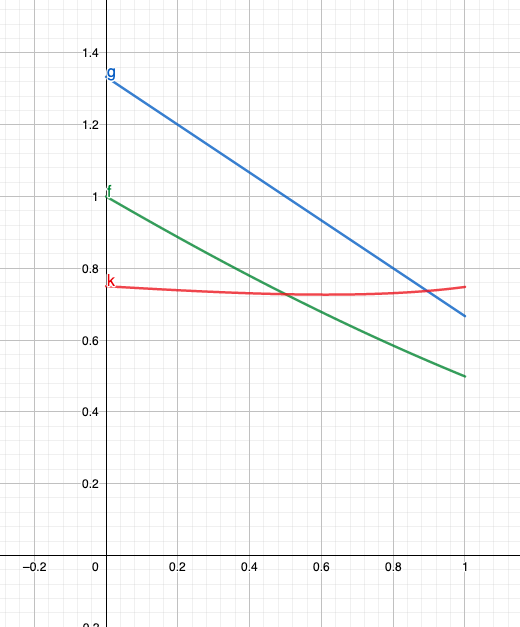
\includegraphics[width=0.3\textwidth]{f_g_fg.png}
\caption{\label{fig:f_g_fg} f em verde, g em azul, e f/g em vermelho, que é aproximadamente constante. }
\end{figure}
\newpage
Para simular $x \sim g(x)$, usaremos o Método da Transformação Inversa. Nossa função de distribuição acumulada entre 0 e 1 será dada por:
\[
G(x) = \int_{0}^{x} g(t) \,dt =  \frac{4x - x^2}{3}
\]
Invertendo G no intervalo selecionado obtemos:
\[
G^{-1}(u) = \frac{4-\sqrt{16-12u}}{2}
\]
$\implies$ Usaremos $x = G^{-1}(u)$, com $u \sim U(0,1)$ para ter $x \sim g$.



\subsection{Método de Monte Carlo 'Control Variate'}
Tomaremos uma função h(x) que é aproxima bem f(x) no intervalo selecionado tal que h(x) é facilmente integrável analiticamente.
Temos então:
\[
\int_{0}^{1} f(x) \,dx = \int_{0}^{1} \PC{f(x) + h(x) - h(x)}  \,dx 
\]
Seja $\gamma`= \int_{0}^{1} h(x)dx  $. Assim, vamos simular $n_4$ valores $x \sim U(0,1)$, e nosso estimador $\widehat{\gamma_4}$ será calculado como:
\[
\widehat{\gamma_4} = \frac{1}{n_4} \sum_{i=1}^{n_4} \PC{f(x_i)-h(x_i)+\gamma`} 
\]
Temos que:
\[ 
E(\widehat{\gamma_4}) = \gamma
\] 
e
\[
\sigma^2_4 = \frac{1}{n} \PR{Var(f(x_i)) + Var(h(x_i)) -2 \rho (f(x_i), h(x_i)) \times
DP(h(x_i)) \times DP(h(x_i)) }
\]
Onde Var é a variância, DP o desvio padrão e $\rho$ a correlação linear.

Usaremos:
\[
h(x) = 1 - \frac{x}{2}
\]
encontrado também 'a olho', e que aproxima f surpeendentemente bem, como mostra a figura 2.
\begin{figure}[ht]
\centering
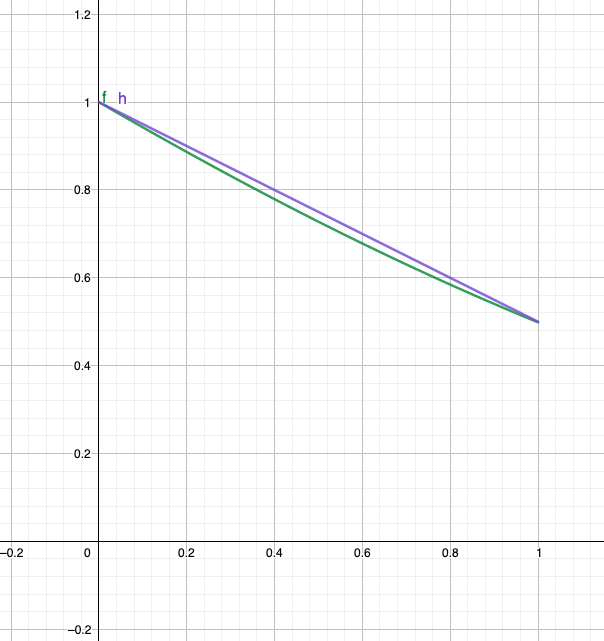
\includegraphics[width=0.35\textwidth]{fh.png}
\caption{\label{fig:fh} f em verde, h em lilás. }
\end{figure}

E temos $\gamma`= \int_{0}^{1} h(x)dx = 0.75 $
\newpage

\section{Calculando os tamanhos de amostra}
\subsection{Erro e confiança}

Já sabemos os métodos para simular $\gamma$, mas se queremos uma aproximação suficientemente boa, temos que ajustar o número de pontos simulados para nos dar certa confiabilidade. Vamos procurar um erro menor ou igual a 0,005\% com confiança de 0,95\%. De acordo com (1), precisamos de 3 valores para achar n: $\varepsilon$, $z_\delta$ e $\sigma$. Esse último muda para cada método, mas vamos calcular os dois primeiros, que se mantêm iguais:

\subsubsection{Calculando $\varepsilon$}
Como o $\varepsilon$ da fórmula (1) é em valor absoluto, temos $\varepsilon = |\widehat{\gamma} - \gamma|$. Queremos o erro percentual de 0,05\% de $\gamma$, ou seja,
\begin{equation}
    \frac{|\widehat{\gamma} - \gamma|}{\gamma} \leq 0,0005 \implies\varepsilon \leq 0,0005 \times \gamma
\end{equation}

Para calcular nosso erro máximo, precisamos de algum limitante inferior de $\gamma$. Vamos analisar f(x):  Como a função exponencial com constante negativa multiplicando x é estritamente decrescente, e como $cos(kx)$ é estritamente decrescente de 0 até $\pi/2k$, e nosso $k<0$, temos a garantia que f(x) é estritamente decrescente pelo menos de 0 até $\pi/2$, intervalo que contém [0,1]. Dado que f é decrescente, vamos usar as somas de Darboux para estimar nosso erro com o python:
\[
M_i = sup(f(x)), x \in [x_{i-1}, x_i] \implies M_i = f(x_i)
\]
e
\[
m_i = inf(f(x)), x \in [x_{i-1}, x_i] \implies m_i = f(x_{i-1})
\]
Assim, vamos usar uma partição uniforme de [0,1] de n=100 elementos e calculamos:

\begin{figure}[ht]
\centering
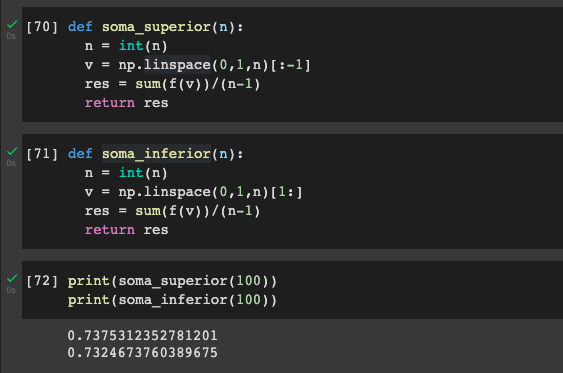
\includegraphics[width=0.8\textwidth]{somaspy.png}
\caption{\label{fig:somaspy} Calculando as somas de Darboux }
\end{figure}
Então vamos chamar esse resultado da soma superior de $S_\gamma$ e o da soma inferior de $I_\gamma$. Temos:
\[
0.7324673760389675 = I_\gamma \leq \gamma \leq S_\gamma = 0.7375312352781201 
\]

Assim, $I_\gamma $ é limitante inferior de $\gamma$, logo se tomarmos $\varepsilon = 0.0005 \times I_\gamma$, temos um erro máximo mais restrito que o planejado, deixando a aproximação mais precisa. \\
$\varepsilon = 0.0005 \times I_\gamma \approx 0.00036623368801948377$



\subsubsection{Calculando $z_\delta$}
Como definimos anteriormente que usariamos uma confiança de 95\%, temos $\delta = 0,95$. Pela tabela da normal: $P(-1,96 \leq Z \leq 1,96) = 0,95 \implies z_\delta = 1,96$.

\subsubsection{Calculando $\sigma^2_2$ e $n_2$}
Vamos começar a calcular os tamanhos de amostra não pelo primeiro, mas pelo segundo método. O motivo disso é que usaremos alguns resultados daqui para calcular a variância do primeiro método. Temos:
\[
\sigma^2_2 = \frac{\gamma(1 - \gamma)}{n_2}
\]
Sabemos que o máximo da função p(1-p) é 0,25; quando p=0,5. Ou seja, o máximo valor que $\sigma^2_2$ é 1/4$n_2$. Como em (1) usamos $\sigma^2$ para quando a variância é $\sigma^2 /n$, temos:
\[
n_2 =  \frac{1,96^2 \times 0.25}{(0,0005 I_\gamma)^2} = 7160371
\]
\subsubsection{Calculando $\sigma^2_1$ e $n_1$}
Para estimar $\sigma^2_1$ vamos usar o seguinte resultado: fixado n, temos:
\[
\sigma^2_2 - \sigma^2_1 = \frac{\gamma(1 - \gamma)}{n} - \frac{1}{n} \int_{0}^{1} (f(x) - \gamma)^2 \,dx  = \frac{1}{n} \PR{\gamma(1 - \gamma) + \gamma^2 - \int_{0}^{1} f(x)^2 \,dx} =  \frac{1}{n} \PR{ \gamma -\int_{0}^{1} f(x)^2 \,dx }
\]
Como sabemos que $0<f(x)\leq 1$, e f(x) $\neq$ 1,  a integral de $f^2(x)$ deve ser menor que a de f(x), com $x \in [0,1]$. Ou seja:
\[
 \frac{1}{n} \PR{ \gamma -\int_{0}^{1} f(x)^2 \,dx } > 0 \implies \sigma^2_2 > \sigma^2_1 \implies \frac{1}{4} > \sigma^2_1
\]
Concluimos que a variância do método 1 é menor que 1/4n, então podemos usar o mesmo n do método 1:
\[
n_1 =  \frac{1,96^2 \times 0.25}{(0,0005 I_\gamma)^2} = 7160371
\]

\subsubsection{Calculando $\sigma^2_3$ e $n_3$}
Temos 
\[
\sigma^2_3 = \frac{1}{n} \int_{0}^{1} (\frac{f(x)}{g(x)} - \gamma)^2 \,g(x)dx =  \int_{0}^{1}\PC{\frac{f^2(x)}{g(x)} - 2\gamma f(x) + \gamma^2 g(x)}\,dx.
\] \\
Como $ \int_{0}^{1} g(x)dx = 1$ e $ \int_{0}^{1} f(x)dx = \gamma$, temos:
\[
\sigma^2_3 = \PR{\int_{0}^{1} \frac{f^2(x)}{g(x)}\,dx} - \gamma^2
\] \\
Sabemos que $g(x)>f(x) \forall x \in [0,1]$ e que $f(x) \leq 1\forall x \in [0,1]$, ou seja:
\[
\frac{f^2(x)}{g(x)} < \frac{f(x)}{g(x)} < f(x) \implies \int_{0}^{1} \frac{f^2(x)}{g(x)}\,dx < \gamma
\]
Então $\gamma - \gamma^2$ é limitante superior da nossa variância, e já mostramos ser limitado superiormente por 0,25:
Assim, usando 0,25 de variância obtemos um $n$ mais preciso:

\[
n_3 =  \frac{1,96^2 \times 0.25}{(0,0005 I_\gamma)^2} = 7160371
\]

\subsubsection{Calculando $\sigma^2_4$ e $n_4$}
Temos que:
\[
\sigma^2_4 = var(f(x)-h(x)) = \int_{0}^{1}(f(x)-h(x) - E(f(x)-h(x)))^2 \,dx = \int_{0}^{1}(f(x)-h(x)-\gamma+0,75)^2 \,dx
\]
Vamos chamar $D(x)=f(x)-h(x)$ e $ k = E(D(x)) = \gamma - 0,75$ 
\[
\sigma^2_4 = \int_{0}^{1}(D(x)-k)^2 \,dx = \int_{0}^{1}D^2(x) \,dx -2k\int_{0}^{1} D(x) \,dx + k^2
\]

Se tomarmos um limitante superior de $\int_{0}^{1}D^2(x) \,dx $, e um inferior de $\int_{0}^{1} D(x)dx$, assim como minimizar o k multiplicando a integral e maximizar o que está elevado ao quadrado, teríamos um limitante superior da variância. Temos que $min(D(x))\approx 0,2233 $ (Imagem 4), então temos:  $\int_{0}^{1} D(x)dx \leq -0,224$ e  $\int_{0}^{1} D^2(x)dx \geq 0,222^2$. Além disso, k = $\gamma -0.75 < 0$ 


\begin{figure}[ht]
\centering
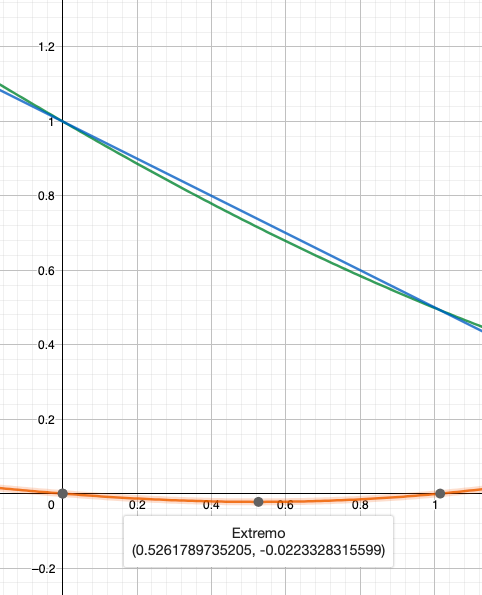
\includegraphics[width=0.335\textwidth]{minimo.png}
\caption{\label{fig:minimo} mínimo de f(x)-h(x) }
\end{figure}


Então para maximizar $k^2$ e minimizar k, pegamos o possível $\gamma$ com maior diferença absoluta de k: $I_\gamma$.
Assim, temos:
\[
\sigma^2_4 \leq 0,222^2 - 2(-0,224)(I_\gamma) + I_\gamma^2
\]
Fazendo isso no python, voltamos com $\sigma^2_4 \leq 0,04173677736841641$. Assim, finalmente:
\[
n_4 =  \frac{1,96^2 \times 0,04173677736841641}{(0,0005 I_\gamma)^2} = 1195404
\]

Assim, temos todos nossos $n_s$ que desejávamos para estimar $\gamma$

\section{Referências}
Bussab \& Morettin - Estatística Básica, $6^a$ edição. Editora Saraiva, 2009.
\\
https://stringfixer.com/pt/Darboux\_integral
\end{document}
